% This is samplepaper.tex, a sample chapter demonstrating the
% LLNCS macro package for Springer Computer Science proceedings;
% Version 2.20 of 2017/10/04
%
\documentclass[runningheads]{llncs}
%
\usepackage{graphicx}
\usepackage{booktabs}
\usepackage{adjustbox}      

% Used for displaying a sample figure. If possible, figure files should
% be included in EPS format.
%
% If you use the hyperref package, please uncomment the following line
% to display URLs in blue roman font according to Springer's eBook style:
% \renewcommand\UrlFont{\color{blue}\rmfamily}

\begin{document}
%
\title{A Study of Herbie effects on FPTaylor computation of error bounds \thanks{Supported by organization x.}}
%
%\titlerunning{Abbreviated paper title}
% If the paper title is too long for the running head, you can set
% an abbreviated paper title here
%
\author{Rocco Salvia, \and
Zvonimir Rakamari\'c}
%
\authorrunning{Salvia et al.}
% First names are abbreviated in the running head.
% If there are more than two authors, 'et al.' is used.
%
\institute{School of Computing, University of Utah, USA \email{rocco@cs.utah.edu}\\ \email{zvonimir@cs.utah.edu}}
%
\maketitle              % typeset the header of the contribution
%
\begin{abstract}
Inexact arithmetic caused by the quantization of real arithmetic into finite representations caused the development of a wide range of academic and industrial tools to both bound and reduce the approximation error. Due to the different research questions faced, it is critical to build interfaces for cooperation among these tools to better succeed in the analysis of approximate computing.
This work describes what the benefits of combining FPTaylor and Herbie, two well known floating-point analyzers, together on the same arithmetic expression. 
FPTaylor is a rigorous estimator of the approximation error deriving from the quantization of real arithmetic into finite arithmetic. FPTaylor detects an upper bound for the maximum error produced by an expression in a bounded numeric interval.
Herbie is a rewriter tool, it rewrites the original expression to reduce the quantization error. Herbie returns a new expression with similar behavior with respect to the original one, but with a lower approximation error. The goal of this work is to empirically verify if Herbie's rewrites always result in a lower error bound in FPTaylor. On the other hand, we verify how FPTaylor can take advantage from Herbie and provide an alternative expression to the user.

\keywords{Herbie, FPTaylor, Floating-point}
\end{abstract}

\section{Introduction} Floating-point arithmetic makes real arithmetic feasible on machines, but it introduces approximation errors both in the conversion and during each computation. In real world computations it has been shown what the effect of approximations error introduced by floating-point arithmetic are on the correct execution of a program. For example, the use of coarse floating-point arithmetic can dramatically impact the results of some critical computations. In the past, there have been incidents caused by insufficient focus towards these approximation problems.

The goal in the analysis of an expression is to bound the maximal approximation error can derive from a finite precision computation. Given the inexact nature of floating-point arithmetic, even small errors may affect the stable flow of a program.

There exist tools providing rigorous error bound estimation for an arithmetic expression together with a proof certificate to support such bound~\cite{fptaylor,magron,precisa,daisy}. FPTaylor~\cite{fptaylor} relies on symbolic Taylor expansions to quantify the error introduced by an arithmetic expression. Taylor expansions approximate the original expression with a summation of polynomials. In this way, the approximation error is a symbolic coefficient of one of the terms in the summation.

In parallel to rigorous estimators, there exist floating-point analyzers looking for the best precision tuning for an expression or a program. Their goal is to minimize the floating-point precision for an expression, e.g. whether the minimal configuration does not affect the accuracy of the result with respect to the original computation~\cite{mixedLam,herbgrind,precimonius}.
Unfortunately, these tools cannot test all possible configurations because of the huge space to scan (from 1 to 52 bits for each of the n variables in a program: it results in a space of $O(52^n)$, that can be drastically reduced to $O(3^n)$ if only half, single or double precision standards from IEEE 754~\cite{ieee} are used for the evaluation). 
The result is that heuristics are adopted without any rigorous guarantees.
Using a similar unsound approach, Herbie~\cite{herbie} is a tool that randomly scans the input domain of a formula to detect sensitive input values producing high floating-point approximation errors. Herbie then rewrites the expression to reduce the floating-point error in specific intervals of the domain. The result is that given an expression, Herbie returns multiple rewrites each one associated to a specific interval of the domain of the expression. Herbie aims to improve the accuracy of the expression in the all domain.

Recent effort in cooperation among  tools result in a parallel project~\cite{daisyherbie} involving Daisy~\cite{daisy} and Herbie~\cite{herbie}. No matter the different tools adopted in the analysis, the main difference with this work concerns the approach used in the evaluation of the final product. In this work we use Herbie as an improvement to FPTaylor capabilities, e.g. as an additional power available in FPTaylor. Indeed our experiments we are focused on the performance of FPTaylor compared to the fusion of FPTaylor with Herbie (FPTherbie). The motivation is mainly due to the different nature of these two analyzers. Herbie does not come with rigorous guarantee unlike the rigorous approach adopted by FPTaylor. In our intension, Herbie is a useful heuristic in addition to FPTaylor, and in this work we evaluate the accuracy of the rewriter.

The overview of this project is shown in Figure\ref{fig:architecture}. Given in input a floating-point expression and a bounded interval, FPTaylor returns the bound of the original expression (flow 1) together with the new bound on the rewritten expression (flow 2). 
Two properties are checked in new tool: (i) verify how FPTaylor can benefit from Herbie in terms of number of reduced bounds and (ii) verify the reliability of Herbie in terms of $accuracy= \frac{lower bounds}{rewritten expressions}$
\begin{figure*}[t]
	\begin{center}
		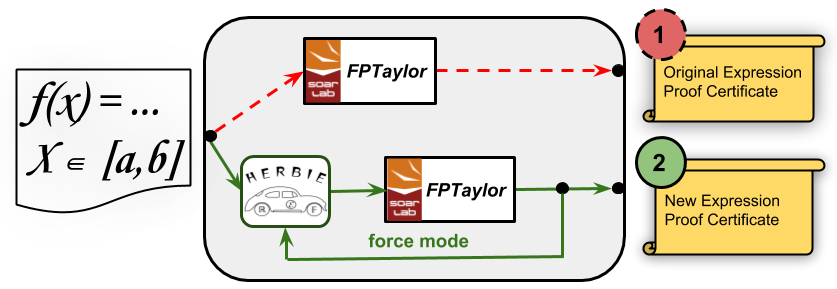
\includegraphics[width=\columnwidth]{picture}
	\end{center}
	\caption{Overview}\label{fig:architecture}
\end{figure*}

\section{Methodology}
In this work we evaluate our tool on the benchmarks\footnote{The benchmarks are available at https://github.com/soarlab/FPTaylor} reported in FPTaylor~\cite{fptaylor} repository. The main issue with Herbie benchmarks is they do not come with a bounded interval for variables in the expression.

In the standard execution flow reported in Fig.~\ref{architecture} the original expression is given as an input to FPTaylor which compute an upper bound for the approximation error generated by the expression. This flow corresponds to flow one in Fig.~\ref{architecture}.
In the second scenario (flow two) (i) Herbie rewrites the expression and (ii) FPTaylor detects the approximation bound of the new expression.

Both Herbie and FPTaylor requires a dedicate format for input expressions. For this reason, this project relies on FPBench\footnote{https://github.com/FPBench/FPBench}, a repository containing formats converters among a variety of floating-point analyzers. 
In particular, FPBench provides a converter from FPTaylor to Herbie format (and vice-versa).

As described in Solovyev et al. FPTaylor does not currently support few operators (actually supported in Herbie) like pow and cbrt (cubic root). The temporary solution adopted for this prototype is to ask Herbie to do not use such operators when improving the expression (with the potential risk of missing the best improvement).

\section{Results}



\begin{table}[h]
	\centering
	\caption{Experimental results for absolute round off errors.}\label{tab1}
	\begin{adjustbox}{center}
	\begin{tabular}{l|c|c|c|c|c|c|c|c|c|}
		&
		\multicolumn{4}{|c|}{Herbie} & \multicolumn{2}{|c|}{FPTaylor}& \multicolumn{3}{|c|}{Stats} \\
		
		\cmidrule{2-5}\cmidrule{5-6}\cmidrule{6-10}
		Name     & \multicolumn{2}{|c|}{Original}   & \multicolumn{2}{|c|}{Rewrite}  & Original & Rewrite & Fail. & Unk. &Illegal \\
		\midrule
		sine &(256 0) & (8000 0.005) &(256 0.0039) & (8000 0.0029)&4.43e-16& FAIL& 0& 0& 3(/0)\\
		sineOrder3 &(256 0.1289) & (8000 0.1347)&(256 0.1289) &(8000 0.1347)& 5.93e-16& 5.93e-16& 0& 0& 0\\
		sqroot&(256 0.01172)& (8000 0.0101)&(256 0.0039) &(8000 0.0098) & 5.01e-16& FAILURE& 0& 20& 0\\
		t\_div\_t1 &(256 0.0195)& (8000 0.0196)&(256 0.01953)& (8000 0.0196)& 2.21e-16 & 2.21e-16 & 0& 0& 0\\
		carbonGas &/&/&/&/& 5.90046e-09 & 5.900398e-09& 0& 0& 0\\
		doppler1 &/&/&/&/& 1.21e-13 & 1.21e-13& 2& 0& 0\\
		doppler2 &(256 0.2936) &(8000 0.3017)&(256 0.2936) &(8000 0.3017)& 2.22e-13 & 2.22e-13 & 2& 1& 1(/0)\\
		doppler3 &/&/&/&/& 6.62e-14 & 6.62e-14 & 2& 0& 0\\
		himmilbeau &/&/&/&/& 1.10e-12 & 1.10e-12 & 0& 0& 0\\
		jetEngine &/&/&/&/& 1.03e-11 & 1.03e-11 & 0& 0& 0\\
		kepler0 &/&/&/&/& 7.46e-14 & 7.46e-14 & 0& 0& 0\\
		kepler1 &/&/&/&/& 2.86e-13 & 2.86e-13 & 0& 0& 1(/0)\\
		kepler2 &/&/&/&/& 1.57e-12 & 1.57e-12 & 0& 0& 0\\
		predPrey &(1024 0.4444) &(8000 0.4210)&(1024 0.4041)& (8000 0.4233)& 1.58e-16 & 1.55e-16 & 2& 10& 0\\
		rigidBody1 &(256 0) &(8000 0.0040)&(256 0) &(8000 0.0040)& 2.94e-13 & 2.77e-13 & 0& 0& 0\\
		rigidBody2 &(256 0.0742) &(8000 0.0696)&(256 0.0625) &(8000 0.0793)& 3.60e-11 & 3.38e-11 & 0& 0& 0\\
		turbine1 &/&/&/&/& 1.66e-14 & 1.66e-14 & 2& 0& 0\\
		turbine2 &(1024 0.5251)& (8000 0.5510)&(1024 0.5638) &(8000 0.5609)& 2.00e-14 & 2.00e-14 & 3& 0& 0\\
		turbine3 &(256 0.3171) &(8000 0.3397)&(256 0.3014) &(8000 0.3393)& 9.57e-15& FAILURE& 0& 0& 3(+$\infty$)\\
		verhulst &(1024 0.3330) &(8000 0.3365)&(1024 0.3211) &(8000 0.3271)& 2.47e-16 & 2.41e-16 & 6& 2& 0\\
		azimuth &(256 0.3979) &(8000 0.3995)&(256 0.3965) &(8000 0.3932)& 8.90e-15 & 8.540799e-15 & 0& 0& 0\\
		hartman &/&/&/&/& 4.60e-15 & 3.48e-15& 2& 0& 0\\
		logexp &(256 0.0117) &(8000 0.0265)&(256 0.0117) &(8000 0.0265)& 1.98e-15& 1.49e-15& 0& 1& 0\\
		sphere &(256 0.0078) &(8000 0.0109)&(256 0.0078) &(8000 0.0109)& 8.10e-15& 7.49e-15& 0& 0& 0\\
		\hline
		&/&/&/&/ & / & / & 21 & 34 &8\\		
		\hline
	\end{tabular}
	\label{tab:table}
\end{adjustbox}
\end{table}



Table.~\ref{tab:table} reports the evaluation of Herbie, FPTaylor and FPTherbie(rewrite and bound) on the original set of benchmarks of FPTaylor~\cite{fptaylor}. As discussed in the introduction, Herbie does not come with rigorous guarantees for the rewritten expression. Herbie evaluates the original and the rewritten expression for a limited set of points (usually 256, 1024, etc), and it reports the average error for the expression as a measure of the quality of the rewrite. While FPTaylor reports a sound upper bound for the expression.
The columns 'Name' reports the name of the benchmark. For both the tools, Table.~\ref{tab:table} reports the error of the original (Original) and the rewritten expression (Rewrite). The column 'Stats' reports: rewrite failures (Fail), unknown rewrites (Unk.) and illegal rewrites(Illegal). Rewrite failures counts how many times Herbie rewrites the expression but FPTaylor proves a larger bound with respect to the original one. Unknown rewrites reports how many times Herbie rewrites the expression using functions not yet supported in FPTaylor (pow, cbrt, etc.). Illegal rewrites reports how many times the rewritten expression contains a potential bug: FPTaylor detects the new expression may result in a division by zero in the given interval. All the illegal rewrites were manually verified in the expression and they are all true positive bugs.
Out of 24 benchmarks, for $\frac{21}{24}$ of them Herbie provides an expression with a bound at least equal to the original one. While for $\frac{9}{24}$ benchmarks Herbie strictly reduces the final error bound of the expression. 
Given the 21 positive results, Herbie needs in average one failing rewrite before improving the expression (a true improvement is when FPTaylor proves newBound <= origBound).
For $\frac{3}{24}$ benchmarks the rewrite does not produce a valid expression. In both 'sine' and 'turbine3' benchmarks all the rewrites contains a bug (with a division by zero expression). 
In case of 'sqroot' all the rewrites from Herbie contain operators unsupported in FPTaylor.

\section{Conclusion}
This work presents a new tool resulting from the combination of Herbie~\cite{herbie} and FPTaylor~\cite{fptaylor}. 
Herbie aims to improve the accuracy of an expression globally in the all domain of the function. Indeed, it randomly samples the given expression to identify where the function suffers the most from approximation error. The main issue coming with Herbie is that profiling might not be accurate enough, resulting in a partial improvement of the function in some intervals, while it degrades the accuracy for others. Due to the unsoundness of the tool, the rewritten expression might not actually reduce the error bound of the original expression and FPTaylor may detect a loss with respect to the original bound. FPTaylor is a rigorous estimator of the approximation error of a function in a given interval. Due to some incompabilities among Herbie and FPTaylor, some rewrites might contains operators not yet supported in FPTaylor. The temporary solution is to ask tfor another expression to Herbie and the risk is to lose the best rewrite because this limitation.
The results shown how Herbie is not efficient on FPTaylor benchmarks. Out of the 24 benchmarks only in $\frac{9}{24}$ Herbie improves the original expression, while in half of them Herbie provides a false positive to FPTaylor.
A future works might be the not trivial task of manually modify Herbie benchmarks and provide a bounded interval for each variable in the expression. If this is the case they can be given in input to FPTaylor. 
It might be that FPTaylor benchmarks are already optimized. Indeed, the challenge for rigorous estimators (FPTaylor~\cite{fptaylor}, Daisy~\cite{daisy}, PRECISA~\cite{precisa}, etc.) is to provide a least upper bound to the true unknown error of a given expression. FPTaylor benchmarks are already challenging to make life hard to estimators looking for a minimal error bound. Since it comes for free, the integration of Herbie in FPTaylor is something appealing for the user. FPTherbie can provide an alternative for the given expression in case of success of the rewrite. 

% ---- Bibliography ----
%
% BibTeX users should specify bibliography style 'splncs04'.
% References will then be sorted and formatted in the correct style.
%
\bibliographystyle{splncs04}
\bibliography{bibfile}
\end{document}
\grid
\grid
\grid
